\chapter{第三部分}
\section{问题概述}
%
%%对问题的直观描述
%
%
%对项目已有代码的阅读和理解
%
%
%解决问题的思路和想法
%
该部分包含第6、7、8小题。

该部分要求我们利用逻辑来帮助智能体实现定位、地图绘制功能,并最终实现SLAM功能。
\section{算法设计}
%
%用自己的语言描述解决问题所使用的算法的原理及功能,设计思路和算法流程图
%
在定位任务中,智能体在初始阶段便会生成一个探索的方案,我们只需要按照该方案执行每一步动作,解析每次行动后得到的感知,将其加入知识库KB中,并
尝试进行定位即可。“尝试定位”是指遍历所有非外侧围墙的位置,如果依据现有的知识库可以推断出智能体(不)在该位置,则将该结论加入知识库中;
吃豆人在某一在满足知识库KB的模型中在特定位置,则该位置是吃豆人可能存在的位置。

在制图任务中,智能体在初始阶段也会生成一个探索的方案,我们只需要按照该方案执行每一步动作,解析每次行动后得到的感知,将其加入知识库KB中,并
尝试进行制图即可。“尝试制图”是指遍历所有非外侧围墙的位置,如果依据现有的知识库可以推断出在该位置(不)是墙壁,则将该结论加入知识库中。
如果一个位置既无法确定墙壁在该位置,也无法确定墙壁不在该位置,则该位置是否存在墙壁待定。

而SLAM,即同时定位和制图,便只需要将定位和制图组合在一起即可,在初始状态,智能体知道它的初始位置,但是并不知道各个墙壁的位置。同时,智能体
的感知器只能获取到智能体邻近区域的墙壁数量。

\begin{algorithm}[H]
    \SetKw{in}{in}
    \SetKw{print}{print}
    \SetKw{range}{range}
    \SetKw{yield}{yield}
    KB = []\;
    \ForAll(\tcp*[h]{在定位任务中,智能体事先知道所有墙壁位置}){wall \in walls}
    {KB.append(wall.wallSentence())}
    \For(\tcp*[h]{实现规划好的计划}){t \in agent.num\_timesteps}
    {
        KB.append(gatherPacInfo(t))\tcp*[h]{收集和吃豆人相关的信息,包含游戏规则、转移公理、感知器公理等}\;
        possible\_locations = updatePacLocation(t,KB)\tcp*[h]{更新关于位置的信息}\;
        agent.moveToNextState(agent.actions[t])\tcp*[h]{执行计划的下一步}\;
        \yield possible\_locations\;
    }
    \caption{localization(agent)}
\end{algorithm}

\begin{algorithm}
    \SetKw{in}{in}
    \SetKw{print}{print}
    \SetKw{range}{range}
    \SetKw{yield}{yield}
    known\_map.initialize()\tcp*[h]{初始化已知地图(所有位置都待确定,除外边框)}\;
    KB = []\;
    KB.append(pacmanInitialLocation)\;
    \For(\tcp*[h]{实现规划好的计划}){t \in agent.num\_timesteps}
    {
        KB.append(gatherPacInfo(t))\tcp*[h]{收集和吃豆人相关的信息,包含游戏规则、转移公理、感知器公理等}\;
        updateWalllocation(KB,known\_map)\tcp*[h]{更新关于各位置墙壁的信息}\;
        agent.moveToNextState(agent.actions[t])\tcp*[h]{执行计划的下一步}\;
        \yield known\_map\;
    }
    \caption{mapping(agent)}
\end{algorithm}

\begin{algorithm}
    \SetKw{in}{in}
    \SetKw{print}{print}
    \SetKw{range}{range}
    \SetKw{yield}{yield}
    known\_map.initialize()\tcp*[h]{初始化已知地图(所有位置都待确定,除外边框)}\;
    KB = []\;
    KB.append(pacmanInitialLocation)\;
    \For(\tcp*[h]{实现规划好的计划}){t \in agent.num\_timesteps}
    {
        KB.append(gatherPacInfo(t))\tcp*[h]{收集和吃豆人相关的信息,包含游戏规则、转移公理、感知器公理等}\;
        updateWalllocation(KB,known\_map)\tcp*[h]{更新关于各位置墙壁的信息}\;
        possible\_locations = updatePacLocation(t,KB)\tcp*[h]{更新关于位置的信息}\;
        agent.moveToNextState(agent.actions[t])\tcp*[h]{执行计划的下一步}\;
        \yield (known\_map,possible\_location)\;
    }
    \caption{slam(agent)}
\end{algorithm}
\section{算法实现}
%
%在算法原理的基础上,结合代码,讲述算法的实现细节、和兴函数、模块输入输出,数据结构定义等内容
%
该部分的算法实现中依赖以下4个辅助函数:
\begin{enumerate}
    \item gatherPacInfo:用于收集和吃豆人相关的各种信息,例如基本游戏规则对应的约束、解析智能体的感知得到的逻辑语句、智能体的行为
    \item addIfEntail:判断已有知识库KB是否蕴含给定结论,如果是,则将该结论添加入知识库中,并放回True,否则返回False
    \item updatePacLocation:遍历所有非外墙位置,如果已有知识库能判断吃豆人(不)在该位置,则将该信息加入知识库中。同时,通过寻找满足的模型来判断吃豆人是否有可能在该位置中
    \item updateWallLocation:遍历所有非外墙位置,如果已有知识库能判断该位置(不)是墙壁,则将该信息加入知识库中,并在known\_map中进行相应的标记。
\end{enumerate}
\begin{lstlisting}[emph={[3]t,KB,agent,sensorModel,successorAxioms,perceptProcessing},emphstyle={[3]\color{vscode_parametercolor}},emph={[4]Expr,SearchProblem,Callable,Node,Actions,Reached,Any,List,Tuple},emphstyle={[4]\color{vscode_classcolor}}]
def gatherPacInfo(t: int, all_coords: List[Tuple], non_outer_wall_coords: List[Tuple], pacphysics_axioms: Callable,
    agent, walls_grid: List[List] = None,
    sensorModel: Callable = None, successorAxioms: Callable = None,
    perceptProcessing: Callable = None) -> Expr:
    new = []
    new.append(pacphysics_axioms(t, all_coords, non_outer_wall_coords, walls_grid, sensorModel, successorAxioms))
    new.append(PropSymbolExpr(agent.actions[t], time=t))
    percepts = agent.getPercepts()
    new.append(perceptProcessing(t, percepts))
    return conjoin(new)

def addIfEntail(KB: list, conclusion: Expr):
    if entails(conjoin(KB), conclusion):
        KB.append(conclusion)
        return True
    return False

def updatePacLocation(t: int, KB: List, non_outer_wall_coords: List[Tuple]):
    possible_locations = []
    for x, y in non_outer_wall_coords:
        addIfEntail(KB, PropSymbolExpr(pacman_str, x, y, time=t))
        addIfEntail(KB, ~PropSymbolExpr(pacman_str, x, y, time=t))
        if findModel(conjoin(KB + [PropSymbolExpr(pacman_str, x, y, time=t)])):
            possible_locations.append((x, y))
    return possible_locations

def updateWallLocation(KB: List, non_outer_wall_coords: List[Tuple],known_map:List[List]):
    for x, y in non_outer_wall_coords:
        if addIfEntail(KB, PropSymbolExpr(wall_str, x, y)):
            known_map[x][y] = 1
        if addIfEntail(KB, ~PropSymbolExpr(wall_str, x, y)):
            known_map[x][y] = 0
\end{lstlisting}
下面是各算法的具体实现,其中略去了部分的已给代码。
\begin{lstlisting}[emph={[3]problem,agent},emphstyle={[3]\color{vscode_parametercolor}},emph={[4]Generator,Expr,SearchProblem,Callable,Node,Actions,Reached,Any,List,Tuple},emphstyle={[4]\color{vscode_classcolor}}]
def localization(problem, agent) -> Generator:
    # 略去已给代码
    KB = []
    KB += [PropSymbolExpr(wall_str, x, y) if (x, y) in walls_list else ~PropSymbolExpr(wall_str, x, y) for x, y in all_coords]
    for t in range(agent.num_timesteps):
        KB.append(gatherPacInfo(t, all_coords, non_outer_wall_coords, pacphysicsAxioms, agent, walls_grid, sensorAxioms, allLegalSuccessorAxioms, fourBitPerceptRules))
        possible_locations = updatePacLocation(t, KB, non_outer_wall_coords)
        agent.moveToNextState(agent.actions[t])
        yield possible_locations

def mapping(problem, agent) -> Generator:
    # 略去已给代码
    KB.append(PropSymbolExpr(pacman_str, pac_x_0, pac_y_0, time=0))
    for t in range(agent.num_timesteps):
        KB.append(gatherPacInfo(t, all_coords, non_outer_wall_coords, pacphysicsAxioms, agent, known_map, sensorAxioms, allLegalSuccessorAxioms, fourBitPerceptRules))
        updateWallLocation( KB, non_outer_wall_coords,known_map)
        agent.moveToNextState(agent.actions[t])
        yield known_map

def slam(problem, agent) -> Generator:
    # 略去已给代码
    KB.append(PropSymbolExpr(pacman_str, pac_x_0, pac_y_0, time=0))
    for t in range(agent.num_timesteps):
        KB.append(gatherPacInfo(t, all_coords, non_outer_wall_coords, pacphysicsAxioms, agent, known_map, SLAMSensorAxioms, SLAMSuccessorAxioms, numAdjWallsPerceptRules))
        updateWallLocation( KB, non_outer_wall_coords,known_map)
        possible_locations = updatePacLocation(t, KB, non_outer_wall_coords)
        agent.moveToNextState(agent.actions[t])
        yield (known_map, possible_locations)
\end{lstlisting}
\section{实验结果}
成功通过Question6,Question7和Question8的全部测试,实验结果截图分别见图\ref{q6},\ref{q7},\ref{q8}。这里的测试样例均是让吃豆人在
规模较小的迷宫中执行对应的任务。
\begin{figure}[htbp]
    \centering
    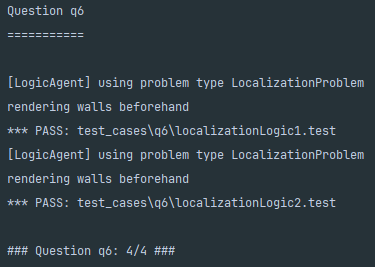
\includegraphics{pic/q6.png}
    \caption{Question6实验结果}\label{q6}
\end{figure}
\begin{figure}[htbp]
    \centering
    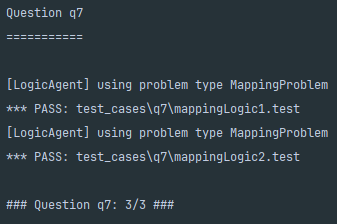
\includegraphics{pic/q7.png}
    \caption{Question7实验结果}\label{q7}
\end{figure}
\begin{figure}[htbp]
    \centering
    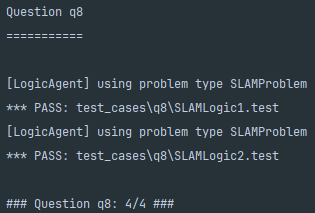
\includegraphics{pic/q8.png}
    \caption{Question8实验结果}\label{q8}
\end{figure}
%
%对试验结果进行详细展示,对每个问题展示测试截图,对于测试用例进行描述说明,对于为通过测试的用例结合自己的算法进行分析,可以结合调试过程进行分析
%
%实验中遇到的问题及解决方案,收获和思考:对算法的理解、优缺点的评价、算法的适用场景
%
